
% =============================================================================
% Project : THE PHILOSOPHY OF VIABILITY
% Book    : Book I — Ontology of Viability
% Book ID : VS.B01
%
% File    :
%   2_MAINMATTER/PART_I_IDENTITY_AND_MANIFESTATION/
%   CHAPTER_08_COMPARATIVE_PHILOSOPHICAL_EXAMINATION/
%   sections/section_02_parmenides.tex
%
% Chapter : 08 — Comparative Philosophical Examination
% Section : 02 — Parmenides
% Structural ID:
%   VS.B01.P01.C08.S02
%
% Purpose :
%   To reconstruct Parmenides' ontology through the surviving
%   fragments and relevant ancient testimonia; distinguish
%   the principal interpretive positions; examine the relation
%   between Being, thought, unity, plurality, change, and the
%   cosmological account; and conduct a reciprocal dialectical
%   examination against the established commitments of
%   Ontology of Viability.
%
% Source Policy:
%   Fragment references follow the Diels–Kranz numbering.
%   Translations and textual claims must be checked against
%   the editions identified in the bibliographic apparatus.
%
% =============================================================================

\section{Parmenides}
\label{sec:ch08-parmenides}

\newcommand{\ParmenidesParagraphAnchor}[1]{%
    \phantomsection\label{para:#1}%
}

\nocite{ParmenidesFragments,CoxonParmenides2009,PalmerParmenides2009,CurdParmenidesSEP,AristotleMetaphysics,AristotlePhysics}

% =============================================================================
% 1. TEXTUAL AND HISTORICAL CONDITIONS
% =============================================================================

\subsection{The Surviving Poem and the Limits of Reconstruction}

\ParmenidesParagraphAnchor{VS.B01.P01.C08.S02.SS01.P001}

Parmenides of Elea is one of the most consequential figures in the
formation of ancient Greek metaphysics. His surviving work presents
a sustained inquiry into what is, what can be thought and said,
and what follows from the conditions under which something is.
The philosophical importance of the poem does not, however,
remove the historical and textual difficulties surrounding its
interpretation. The original work has not survived as a complete
manuscript. Its extant passages are preserved principally through
quotations and reports transmitted by later authors. The text
available to contemporary readers is therefore a reconstruction
whose fragments differ in length, context, and degree of textual
security.

\ParmenidesParagraphAnchor{VS.B01.P01.C08.S02.SS01.P002}

The conventional title \textit{On Nature} should not be treated
as certainly authorial. Nor should the traditional division of
the poem into Proem, Aletheia, and Doxa be mistaken for a division
whose original form is known in every detail. These designations
are useful scholarly conventions for identifying the poem's
principal movements. They do not eliminate uncertainty about
the original sequence, the relation among the fragments, or the
extent to which later transmitters shaped the evidence through
their own philosophical purposes.

\ParmenidesParagraphAnchor{VS.B01.P01.C08.S02.SS01.P003}

The textual problem is philosophically relevant. A reconstruction
of Parmenides must distinguish direct poetic fragments from
testimonia: reports, summaries, interpretations, and arguments
attributed to him by later authors. A statement preserved as a
verbatim fragment does not have the same evidential status as a
later author's account of what Parmenides supposedly maintained.
The latter may preserve valuable information, but it must be
examined in relation to the philosophical interests and conceptual
vocabulary of the transmitter. In particular, Aristotle's
classification of Parmenides alongside Melissus is historically
important, but it must not be treated as an unmediated statement
of Parmenides' own theoretical architecture.

\ParmenidesParagraphAnchor{VS.B01.P01.C08.S02.SS01.P004}

The present examination therefore adopts three methodological
restrictions. First, the surviving fragments constitute the
primary textual basis for reconstructing Parmenides' position.
Second, ancient testimonia are used as evidence about reception,
historical interpretation, and otherwise lost material, but
their claims are not automatically attributed to Parmenides.
Third, modern interpretations are treated as competing
reconstructions rather than as interchangeable summaries of
an uncontested doctrine.

\ParmenidesParagraphAnchor{VS.B01.P01.C08.S02.SS01.P005}

The distinction between textual evidence and philosophical
interpretation is especially important because the central
questions remain disputed: whether Parmenides advances strict
numerical monism; whether his principal argument concerns
existence, predication, necessity, or the conditions of
intelligible inquiry; whether the mortal cosmology is wholly
rejected or possesses a qualified explanatory status; and
whether the poem's account of what-is is intended to describe
one unique entity or the necessary character of whatever
genuinely is. These questions must remain visible throughout
the comparison.


% =============================================================================
% Project : THE PHILOSOPHY OF VIABILITY
% Book    : Book I — Ontology of Viability
% Book ID : VS.B01
% Chapter : 08 — Comparative Philosophical Examination
% Section : 02 — Parmenides
%
% Asset ID:
%   VS.B01.P01.C08.S02.SS01.P003.IL01
%
% Type    : IL — Illustration
% File    : threshold_of_inquiry.tex
%
% Purpose :
%   Provide a restrained symbolic illustration of the threshold
%   imagery in the proem of Parmenides' poem. The image is
%   interpretive and atmospheric, not a historical reconstruction
%   or a diagram of the poem's philosophical argument.
% =============================================================================

\begin{figure}[htbp]
\centering

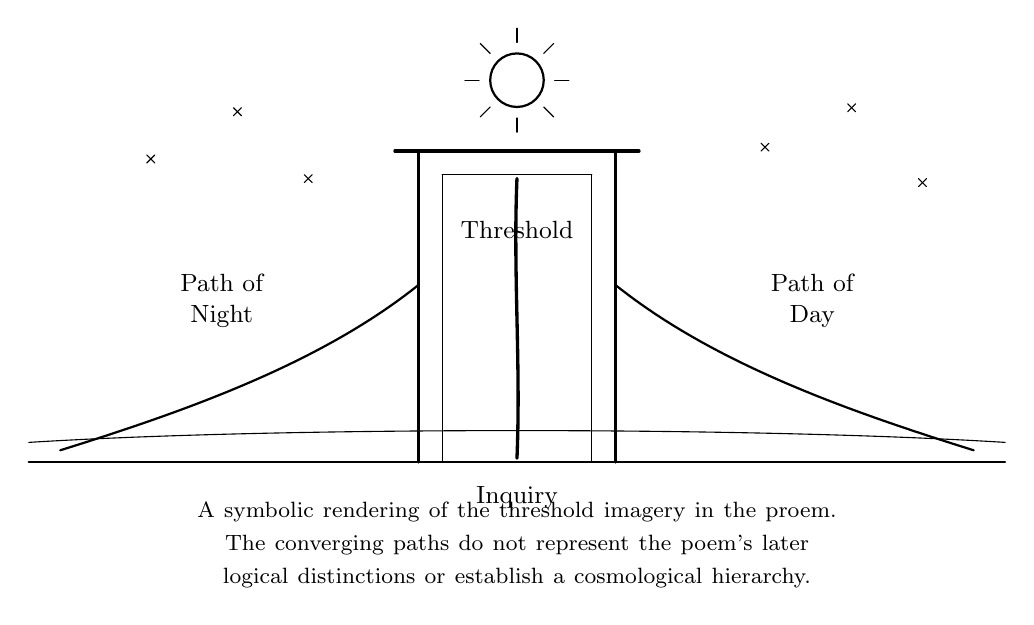
\begin{tikzpicture}[
    line cap=round,
    line join=round,
    scale=1.0
]

% Ground and horizon
\draw[thick] (-6.2,-2.4) -- (6.2,-2.4);
\draw[thin] (-6.2,-2.15) .. controls (-3.0,-1.95)
    and (3.0,-1.95) .. (6.2,-2.15);

% Threshold structure
\draw[very thick] (-1.25,-2.4) -- (-1.25,1.55);
\draw[very thick] (1.25,-2.4) -- (1.25,1.55);
\draw[very thick] (-1.55,1.55) -- (1.55,1.55);

% Inner gate lines
\draw[thin] (-0.95,-2.4) -- (-0.95,1.25);
\draw[thin] (0.95,-2.4) -- (0.95,1.25);
\draw[thin] (-0.95,1.25) -- (0.95,1.25);

% Two paths approaching the threshold
\draw[thick]
    (-5.8,-2.25)
    .. controls (-4.2,-1.75) and (-2.5,-1.15)
    .. (-1.25,-0.15);

\draw[thick]
    (5.8,-2.25)
    .. controls (4.2,-1.75) and (2.5,-1.15)
    .. (1.25,-0.15);

% Central path beyond the gate
\draw[very thick]
    (0,-2.35)
    .. controls (0.05,-1.15) and (-0.05,0.0)
    .. (0,1.2);

% Sun and stars
\draw[thick] (0,2.45) circle (0.34);
\foreach \a in {0,45,...,315}{
    \draw[thin]
        ({0.48*cos(\a)},{2.45+0.48*sin(\a)})
        --
        ({0.66*cos(\a)},{2.45+0.66*sin(\a)});
}

\foreach \x/\y in {-4.7/1.4,-3.6/2.0,-2.7/1.15,
                    3.1/1.55,4.2/2.05,5.1/1.1}{
    \draw[thin] (\x,\y) -- ++(0.10,0.10);
    \draw[thin] (\x+0.10,\y) -- ++(-0.10,0.10);
}

% Labels
\node[align=center] at (-3.75,-0.35)
    {\small Path of\\[-1pt]\small Night};

\node[align=center] at (3.75,-0.35)
    {\small Path of\\[-1pt]\small Day};

\node[align=center] at (0,0.55)
    {\small Threshold};

\node[align=center] at (0,-2.85)
    {\small Inquiry};

% Caption note within the illustration
\node[align=center,text width=10.5cm] at (0,-3.45)
    {\footnotesize
    A symbolic rendering of the threshold imagery in the proem.
    The converging paths do not represent the poem's later
    logical distinctions or establish a cosmological hierarchy.};

\end{tikzpicture}

\caption{The Threshold of Inquiry in the Proem of Parmenides}
\label{fig:ch08-parmenides-threshold}

\end{figure}

% =============================================================================
% END OF ASSET
% =============================================================================


\footnote{For the state of the surviving evidence and the distinction
between fragments and testimonia, see A. H. Coxon, \textit{The Fragments
of Parmenides}, revised and expanded edition (2009), Introduction and
the collection of ancient testimonia; David Gallop, \textit{Parmenides
of Elea: Fragments} (1984); and Patricia Curd, ``Parmenides,''
\textit{Stanford Encyclopedia of Philosophy}, substantive revision
4 March 2025, section 1. References to fragments below follow the
Diels--Kranz numbering, DK 28 B.}

% =============================================================================
% 2. THE PROEM AND THE WAYS OF INQUIRY
% =============================================================================

\subsection{The Proem and the Structure of Inquiry}

\ParmenidesParagraphAnchor{VS.B01.P01.C08.S02.SS02.P001}

The poem begins with a proem in which the speaker describes a
journey conducted by divine guides to the abode of a goddess.
The imagery includes a chariot, the daughters of the Sun, the
gates of the paths of Night and Day, and the figure of Justice
who guards their passage. The goddess receives the traveller
and announces that he must learn both the unshaken account of
truth and the opinions of mortals. The proem is not merely an
ornamental introduction. It establishes the dramatic and
didactic setting in which the poem's subsequent distinctions
are presented.

\ParmenidesParagraphAnchor{VS.B01.P01.C08.S02.SS02.P002}

The proem should not be reduced to a simple allegory in which
the journey represents the movement of an individual mind from
ignorance to knowledge. Its imagery belongs to a wider archaic
poetic and religious environment, and its interpretation requires
attention to the cultural and literary forms through which the
poem presents philosophical instruction. The journey gives
the revelation a distinctive authority within the poem, but
the arguments that follow must still be assessed by their
content and inferential force. Divine presentation is not
a substitute for philosophical reconstruction.

\ParmenidesParagraphAnchor{VS.B01.P01.C08.S02.SS02.P003}

Fragment B2 introduces two ways of inquiry. The first concerns
that it is and that it cannot not be; the second concerns that
it is not and that it must not be. The goddess rejects the
second way as incapable of yielding knowledge or a reportable
object of inquiry. The contrast is not merely between two
opinions about an already identified object. It concerns
the conditions under which inquiry can have an intelligible
and determinate subject. The first way is associated with
conviction and truth, whereas the second is presented as
unavailable to successful inquiry.

\ParmenidesParagraphAnchor{VS.B01.P01.C08.S02.SS02.P004}

The expression translated as ``what-is'' is philosophically
significant and textually difficult. The Greek forms of the
verb \textit{einai} may support existential, predicative,
veridical, or other contextually related readings. The poem
does not provide a modern technical definition that settles
these possibilities in advance. Consequently, the translation
of the relevant expressions as ``Being,'' ``what is,'' or
``that which is'' must not be allowed to decide the
interpretation before the argument has been examined.

\ParmenidesParagraphAnchor{VS.B01.P01.C08.S02.SS02.P005}

Fragment B3 is frequently invoked in discussions of the relation
between thinking and being. Its compressed formulation has
generated disagreement concerning whether it expresses an
identity, a necessary correlation, a condition of intelligibility,
or a relation between what can be thought and what can be.
Whatever interpretation is preferred, the fragment must not
be converted without argument into the general thesis that
Being depends upon cognition. The poem's relation between
thought and what-is is part of its own philosophical problem;
it does not by itself establish that existence is constituted
by an act of knowing.

\ParmenidesParagraphAnchor{VS.B01.P01.C08.S02.SS02.P006}

Fragments B6 and B7 complicate the apparently exhaustive
division introduced in B2. B6 describes the path followed
by mortals who fail to distinguish being and not-being
adequately and whose thought wanders. This path is not
straightforwardly identical with the impossible route
of absolute non-being in B2. It involves a confused
intermingling or unstable treatment of being and not-being.
The distinction between these passages has led influential
interpreters to recognize a third way of inquiry, distinct
from both the path of necessary being and the impossible
path of what cannot be.

\ParmenidesParagraphAnchor{VS.B01.P01.C08.S02.SS02.P007}

The structure of inquiry can therefore be represented through
three distinguishable routes: the route of what-is and cannot
not be; the route of what-is-not and cannot be; and the
confused mortal route that treats being and not-being without
adequate discrimination. The third route is not simply a
successful alternative to the first. It is associated with
the unstable judgments of mortals. Nevertheless, its presence
is essential for understanding why the poem contains a
substantial cosmological account after the argument concerning
what-is.

% =============================================================================
% Project : THE_PHILOSOPHY_OF_VIABILITY
% Book    : Book I — Ontology of Viability
% Book ID : VS.B01
% Part    : Part I — Identity and Manifestation (VS.B01.P01)
% Chapter : Chapter 08 — Comparative Philosophical Examination
% Chapter ID : VS.B01.P01.C08
%
% File    : 4_ASSETS/figures/VS.B01.P01.C08.S02.SS02.P004.FG01.structure_of_parmenides_poem.tex
%
% Section / Chapter / Asset:
%   Figure FG01 — Structure of Parmenides' Poem
%
% Structural Identifier : VS.B01.P01.C08.S02.SS02.P004.FG01
% Asset Type : FG
%
% Purpose :
%   To represent the principal textual movements of Parmenides' poem and to
%   make visible the interpretive problem concerning the relation between
%   Aletheia and Doxa.
%
% Representational limit :
%   The diagram follows the sequence of the text; it does not settle the
%   interpretive dispute concerning the relation between Aletheia and Doxa.
%
% Dependencies :
%   TikZ; libraries used: arrows.meta, calc, positioning. All are loaded by
%   the project preamble; no per-file package or library loading.
%
% =============================================================================

\begin{figure}[htbp]
    \centering
    \hyphenpenalty=10000 \exhyphenpenalty=10000\relax  % no hyphenation inside diagram labels

    \begin{tikzpicture}[
        font=\small,
        node distance=1.0cm,
        % --- base box ---
        box/.style={
            draw, rounded corners=3pt, align=center,
            text width=4.2cm, minimum height=1.4cm,
            inner sep=5pt, line width=0.7pt
        },
        % --- node roles ---
        movement/.style={box, fill=blue!8, draw=blue!55!black},
        openbox/.style={box, text width=9.6cm, dashed, fill=gray!10,
                        draw=black!60},
        % --- arrows and labels ---
        directed/.style={-{Stealth[length=2.5mm]}, line width=0.9pt},
        disputed/.style={-{Stealth[length=2.5mm]}, line width=0.9pt, dashed},
        elabel/.style={font=\footnotesize\itshape, text=black!75,
                       align=center, text width=2.4cm}
    ]

    % ---------------------------------------------------------------
    % Textual sequence
    % ---------------------------------------------------------------
    \node[movement] (proem) {
        \textbf{Proem}\\[2pt]
        Journey, gates, divine reception
    };
    \node[movement, below=of proem] (program) {
        \textbf{Program of Revelation}\\[2pt]
        Truth and mortal opinions
    };

    % ---------------------------------------------------------------
    % The two principal accounts
    % ---------------------------------------------------------------
    \node[movement] (aletheia) at ($(program)+(-3.0,-3.0)$) {
        \textbf{Aletheia}\\[2pt]
        What-is and the deductions of B8
    };
    \node[movement] (doxa) at ($(program)+(3.0,-3.0)$) {
        \textbf{Doxa}\\[2pt]
        Cosmological account and mortal naming
    };

    % ---------------------------------------------------------------
    % Interpretive problem
    % ---------------------------------------------------------------
    \coordinate (accounts) at ($(aletheia)!0.5!(doxa)$);
    \node[openbox, below=2.2cm of accounts] (problem) {
        \textbf{Interpretive Problem}\\[2pt]
        What is the ontological and explanatory relation between the
        two accounts?
    };

    % ---------------------------------------------------------------
    % Relations
    % ---------------------------------------------------------------
    \draw[directed] (proem)   -- (program);
    \draw[directed] (program) -- (aletheia);
    \draw[directed] (program) -- (doxa);
    \draw[disputed] (aletheia.south) -- (aletheia.south |- problem.north)
        node[elabel, midway, right=4pt] {relation disputed};
    \draw[disputed] (doxa.south) -- (doxa.south |- problem.north)
        node[elabel, midway, left=4pt] {status disputed};

    % ---------------------------------------------------------------
    % Legend
    % ---------------------------------------------------------------
    \node[below=0.6cm of problem, font=\scriptsize] {
        \tikz[baseline=-0.5ex]\draw[directed] (0,0) -- (0.7,0);~sequence of the text
        \quad\quad
        \tikz[baseline=-0.5ex]\draw[disputed] (0,0) -- (0.7,0);~relation open to interpretive dispute
    };

    \end{tikzpicture}

    \caption{The principal textual movements of Parmenides' poem. The solid
    arrows follow the sequence of the text; the dashed arrows mark
    the relation between Aletheia and Doxa, which remains a matter
    of interpretive dispute.}
    \label{fig:ch08-parmenides-poem-structure}
\end{figure}

% =============================================================================
% END OF FIGURE FG01
% =============================================================================


\footnote{See Parmenides, DK 28 B1.28--32, B2.1--8, B3, B6.1--9,
and B7.1--6. For the distinction between the two ways of B2
and the mortal route of B6, see John Palmer, \textit{Parmenides
and Presocratic Philosophy} (2009), chapters 2--3, and Curd,
``Parmenides,'' sections 2.2 and 3.5.}

% =============================================================================
% 3. WHAT-IS AND THE DEDUCTIVE SIGNS
% =============================================================================

\subsection{What-Is and the Deductions of Fragment 8}

\ParmenidesParagraphAnchor{VS.B01.P01.C08.S02.SS03.P001}

Fragment B8 develops the principal argument concerning what-is.
The goddess states that a single account remains: that it is.
Along this route, she identifies a series of signs or marks
associated with what-is, including that it is ungenerated,
imperishable, whole, of a single kind, unmoving, and complete.
These descriptions are not introduced as independent
observations about an ordinary object. They are presented
as consequences or necessary characteristics associated
with the route of inquiry that affirms what-is.

\ParmenidesParagraphAnchor{VS.B01.P01.C08.S02.SS03.P002}

The argument against generation and destruction begins from
the difficulty of treating what-is as having arisen from
what-is-not or as passing into what-is-not. If what-is
cannot be derived from what-is-not, generation cannot
be explained through an absolute transition from non-being
to being. If what-is cannot become what-is-not, destruction
cannot be understood as an absolute transition into
non-being. The conclusion is that what-is is not subject
to generation or annihilation in the sense excluded
by the argument.

\ParmenidesParagraphAnchor{VS.B01.P01.C08.S02.SS03.P003}

The argument concerning time is closely related. Parmenides
rejects the characterization of what-is as something that
once was but is no longer, or as something that will be
but is not yet. The argument is commonly interpreted
as excluding temporal coming-to-be and passing-away.
Whether it establishes timeless eternity or uninterrupted
existence is a further interpretive question. The two
claims should not be treated as equivalent without
examining the temporal language and argumentative
context of the fragment.

\ParmenidesParagraphAnchor{VS.B01.P01.C08.S02.SS03.P004}

Fragment B8 also denies division and presents what-is
as continuous and uniform. The argument appeals to
the absence of a differentiating non-being that could
interrupt or separate what-is from itself. The passage
does not merely assert that the whole is assembled
from homogeneous parts. It denies that a division
can be established through a region or condition
of non-being. The precise ontological force of this
reasoning depends upon how the terms of being,
division, and continuity are interpreted.

\ParmenidesParagraphAnchor{VS.B01.P01.C08.S02.SS03.P005}

The argument concerning motion and change follows a
related pattern. What-is is described as remaining
within the limits of powerful necessity, unmoved
and complete. If motion or alteration requires that
what-is cease to be what it is, or that it pass through
what-is-not, such change appears incompatible with
the conditions already established. The conclusion
is not merely that no change has been observed.
It is that the relevant conception of change cannot
be reconciled with the mode of being assigned to
what-is.

\ParmenidesParagraphAnchor{VS.B01.P01.C08.S02.SS03.P006}

The deductions concerning wholeness, uniformity,
continuity, and completeness must nevertheless be
distinguished from one another. A claim that what-is
is whole does not automatically establish that it
is numerically one in every relevant sense. A claim
that it is continuous does not by itself settle
whether it is composed or non-composed. A claim
that it is uniform does not independently determine
the number of identities that may exist. Each
conclusion requires the specific argument by which
Parmenides attempts to establish it.

\ParmenidesParagraphAnchor{VS.B01.P01.C08.S02.SS03.P007}

The spherical image near the end of the principal
deduction is also significant. The goddess compares
what-is to the mass of a well-rounded sphere, equally
balanced from its centre in every direction. This
description has often been understood as a physical
or spatial characterization. Its precise role remains
disputed, especially in relation to interpretations
that treat what-is as an abstract metaphysical
principle. The image must not be detached from
the assumptions about spatiality and completeness
that govern the argument.

\ParmenidesParagraphAnchor{VS.B01.P01.C08.S02.SS03.P008}

The sequence of fragment B8 is therefore an
inferential construction rather than a list of
unrelated attributes. The route of what-is constrains
what may consistently be said of it. Generation,
destruction, division, motion, and incompleteness
are excluded insofar as they require a transition
or condition incompatible with what-is. The
strength of the deductions depends upon whether
the relevant conceptions of non-being, change,
and predication are adequately established.

% =============================================================================
% Project : THE_PHILOSOPHY_OF_VIABILITY
% Book    : Book I — Ontology of Viability
% Book ID : VS.B01
% Part    : Part I — Identity and Manifestation (VS.B01.P01)
% Chapter : Chapter 08 — Comparative Philosophical Examination
% Chapter ID : VS.B01.P01.C08
%
% File    : 4_ASSETS/diagrams/VS.B01.P01.C08.S02.SS03.P006.DG01.parmenidean_routes_and_deduction.tex
%
% Section / Chapter / Asset:
%   Diagram DG01 — Parmenidean Routes and Deduction
%
% Structural Identifier : VS.B01.P01.C08.S02.SS03.P006.DG01
% Asset Type : DG
%
% Purpose :
%   To distinguish the two ways introduced in B2 from the mortal route in B6,
%   and to represent the inferential movement from the affirmation of what-is
%   to the principal signs in B8.
%
% Representational limit :
%   The solid arrows mark the argumentative movement; the dashed arrows mark
%   routes that the poem presents as unavailable or unstable. The
%   reconstruction does not settle the interpretive disputes concerning the
%   fragments.
%
% Dependencies :
%   TikZ; libraries used: arrows.meta, calc, positioning, fit. All are loaded
%   by the project preamble; no per-file package or library loading.
%
% =============================================================================

\begin{figure}[htbp]
    \centering
    \hyphenpenalty=10000 \exhyphenpenalty=10000\relax  % no hyphenation inside diagram labels

    \begin{tikzpicture}[
        font=\small,
        node distance=0.8cm,
        % --- base box ---
        box/.style={
            draw, rounded corners=3pt, align=center,
            text width=3.6cm, minimum height=1.5cm,
            inner sep=5pt, line width=0.7pt
        },
        % --- node roles ---
        route/.style={box, fill=blue!8, draw=blue!55!black},
        deduction/.style={box, fill=blue!16, draw=blue!55!black,
                          minimum height=1.3cm},
        sign/.style={box, fill=green!8, draw=green!40!black,
                     minimum height=1.0cm},
        excluded/.style={box, dashed, fill=gray!10, draw=black!60,
                         minimum height=1.3cm},
        % --- frames and labels ---
        vsgroup/.style={draw=black!45, dashed, rounded corners=5pt,
                        inner sep=8pt, line width=0.5pt},
        grouplabel/.style={font=\footnotesize\itshape, text=black!75,
                           align=center},
        % --- arrows ---
        directed/.style={-{Stealth[length=2.5mm]}, line width=0.9pt},
        optional/.style={-{Stealth[length=2.5mm]}, line width=0.9pt, dashed}
    ]

    % ---------------------------------------------------------------
    % Ways of inquiry (B2) and the mortal route (B6)
    % ---------------------------------------------------------------
    \node[route] (being) {
        \textbf{B2: What-is}\\[2pt]
        It is and cannot not be
    };
    \node[route, right=0.8cm of being] (nonbeing) {
        \textbf{B2: What-is-not}\\[2pt]
        It is not and must not be
    };
    \node[route, right=0.8cm of nonbeing] (mortal) {
        \textbf{B6: Mortal route}\\[2pt]
        Confused treatment of being and not-being
    };
    \node[vsgroup, fit=(being)(nonbeing)(mortal)] (routes) {};
    \node[grouplabel, above=0.1cm of routes] {Ways of inquiry};

    % ---------------------------------------------------------------
    % Consequences of each route
    % ---------------------------------------------------------------
    \node[deduction, below=1.3cm of being] (b8) {
        \textbf{B8: Deduction}\\[2pt]
        What-is must be
    };
    \node[excluded, below=1.3cm of nonbeing] (unavailable) {
        \textbf{Not available}\\[2pt]
        No attainable object of inquiry
    };
    \node[excluded, below=1.3cm of mortal] (wandering) {
        \textbf{Wandering inquiry}\\[2pt]
        Unstable judgment
    };

    % ---------------------------------------------------------------
    % Principal signs of what-is (B8)
    % ---------------------------------------------------------------
    \node[sign, below=1.3cm of b8] (s1) {Ungenerated and imperishable};
    \node[sign, below=0.3cm of s1] (s2) {Whole and continuous};
    \node[sign, below=0.3cm of s2] (s3) {Unmoved and complete};
    \node[vsgroup, fit=(s1)(s2)(s3)] (signs) {};
    \node[grouplabel, right=0.2cm of signs, anchor=west, text width=2.6cm,
          align=left] {Principal signs of what-is (B8)};

    % ---------------------------------------------------------------
    % Relations
    % ---------------------------------------------------------------
    \draw[directed] (being)   -- (b8);
    \draw[directed] (b8)      -- (signs);
    \draw[optional] (nonbeing) -- (unavailable);
    \draw[optional] (mortal)   -- (wandering);

    % ---------------------------------------------------------------
    % Legend and interpretive caution
    % ---------------------------------------------------------------
    \coordinate (axis) at (nonbeing |- signs.south);
    \node[below=0.5cm of axis, font=\scriptsize] (legend) {
        \tikz[baseline=-0.5ex]\draw[directed] (0,0) -- (0.7,0);~argumentative movement
        \quad\quad
        \tikz[baseline=-0.5ex]\draw[optional] (0,0) -- (0.7,0);~route presented as unavailable or unstable
    };
    \node[below=0.35cm of legend, text width=11cm, align=center,
          font=\footnotesize\itshape] {
        The relation between the mortal route, the deductions concerning
        what-is, and the cosmology of Doxa remains a matter of
        interpretation. The mortal route is not equated with absolute
        non-being.
    };

    \end{tikzpicture}

    \caption{The ways of inquiry in B2 and B6 and the deductive structure
    of B8. The solid arrows mark the argumentative movement; the
    dashed arrows mark routes that the poem presents as
    unavailable or unstable. The reconstruction does not settle
    the interpretive disputes concerning the fragments.}
    \label{fig:ch08-parmenides-routes-deduction}
\end{figure}

% =============================================================================
% END OF DIAGRAM DG01
% =============================================================================


\footnote{See DK 28 B8.1--21 for the argument concerning generation
and destruction; B8.22--25 for continuity and uniformity;
B8.26--33 for immobility; and B8.42--49 for completeness and
the spherical comparison. The interpretation of B8.5--6 as
timeless existence or uninterrupted existence remains disputed.
For discussion of the textual arrangement and interpretive
alternatives, see Curd, ``Parmenides,'' sections 2.3 and 3.}

% =============================================================================
% 4. UNITY, WHOLENESS, AND PLURALITY
% =============================================================================

\subsection{Unity, Wholeness, and the Problem of Plurality}

\ParmenidesParagraphAnchor{VS.B01.P01.C08.S02.SS04.P001}

Parmenides' account of what-is has frequently been
interpreted as a defence of strict monism: the thesis
that exactly one entity exists and that plurality
is wholly unreal. This interpretation draws support
from the language of unity, continuity, homogeneity,
and completeness in fragment B8. It also reflects
the difficulty of reconciling the denial of division
and change with the apparent plurality of ordinary
existents. Nevertheless, the conclusion that
Parmenides explicitly establishes the numerical
singularity of all reality requires more argument
than the mere presence of unified or whole language.

\ParmenidesParagraphAnchor{VS.B01.P01.C08.S02.SS04.P002}

Several questions must be distinguished. Does
Parmenides claim that there is only one existent?
Does he claim that whatever genuinely is must
possess a unified and complete character? Does
he deny that several entities can each satisfy
the conditions of what-is? Does he deny plurality
because it requires absolute non-being, or because
he understands difference as incompatible with
the nature of what-is? These are related but
not identical questions. A strict monist answer
to the first question does not follow automatically
from every possible answer to the others.

\ParmenidesParagraphAnchor{VS.B01.P01.C08.S02.SS04.P003}

A distinction between numerical monism and
predicational or essentialist readings is therefore
necessary. On a strict numerical monist reading,
the argument establishes that only one entity
exists. On an essentialist reading, the argument
may instead establish that whatever genuinely
is must possess certain necessary characteristics.
On the latter interpretation, a plurality of
entities may remain possible if each satisfies
the conditions derived in B8. The disagreement
concerns the scope of the subject to which the
deductions apply and the force of the singular
language used in the poem.

\ParmenidesParagraphAnchor{VS.B01.P01.C08.S02.SS04.P004}

The distinction between unity and plurality
must not be resolved by treating every form
of multiplicity as equivalent. A plurality of
components, a plurality of determinations,
a plurality of manifestations, a plurality of
existents, and a plurality of identities are
different ontological questions. Parmenides'
arguments may challenge one or more of these
forms without thereby establishing that every
possible form of plurality is impossible.

\ParmenidesParagraphAnchor{VS.B01.P01.C08.S02.SS04.P005}

Nor should the language of wholeness be
interpreted as equivalent to composition.
A whole may be conceived as an aggregate
of parts, a composition constituted through
relations among components, or a unified
existent whose unity is not explained by
aggregation. Parmenides' denial of division
does not automatically identify which of
these concepts of wholeness is intended.
The relevant question is whether the poem's
argument establishes a particular ontological
form of unity or excludes only those forms
of plurality that require a passage through
absolute non-being.

\ParmenidesParagraphAnchor{VS.B01.P01.C08.S02.SS04.P006}

The question must therefore remain open
until the inferential scope of B8 has been
established. The strict monist interpretation
is a serious and historically influential
reading, but it is not a neutral starting
assumption. Likewise, the essentialist or
modal interpretation cannot be treated as
settled merely because it allows a more
accommodating account of plurality. Both
readings must explain the poem's language,
its deductions, and its cosmological account.

% =============================================================================
% 5. DOXA AND THE COSMOLOGICAL ACCOUNT
% =============================================================================

\subsection{The Cosmological Account and the Status of Doxa}

\ParmenidesParagraphAnchor{VS.B01.P01.C08.S02.SS05.P001}

At the end of fragment B8, the goddess announces
a transition from the trustworthy account of
what-is to the arrangement of mortal opinions.
The surviving fragments that follow contain
a cosmological account involving the principles
of Light and Night, the celestial order, the
Moon, the Sun, the stars, the Earth, and aspects
of biological generation. The presence of this
material creates one of the central interpretive
problems of the poem: why does a philosopher
who has apparently excluded generation, motion,
and plurality devote a substantial portion
of the work to explaining a world characterized
by these very phenomena?

\ParmenidesParagraphAnchor{VS.B01.P01.C08.S02.SS05.P002}

One influential answer treats Doxa as an
account of a world that is wholly unreal or
deceptive. On this interpretation, the
cosmology illustrates the mistaken commitments
of mortals, whose judgments confuse being
and not-being. This reading preserves a
sharp opposition between the truth of what-is
and the apparent world of ordinary experience.
Its difficulty is explaining why the poem
contains such an extensive and technically
detailed cosmology if the account has no
meaningful explanatory role.

\ParmenidesParagraphAnchor{VS.B01.P01.C08.S02.SS05.P003}

Other interpretations assign Doxa a more
qualified status. It may be understood as
a cosmological account of the world as it
appears under mortal conditions, an account
whose explanatory achievements remain
subordinate to the truth concerning what-is.
Some readings distinguish the necessary
mode of being from contingent or changeable
modes of being. Others understand the
cosmology as a systematic account of the
phenomenal world without granting it the
same degree of truth or necessity as the
first part of the poem.

\ParmenidesParagraphAnchor{VS.B01.P01.C08.S02.SS05.P004}

The surviving evidence does not warrant
a simple conclusion that Doxa is either
wholly worthless or fully equivalent in
truth-status to Aletheia. The goddess
explicitly marks a difference in trustworthiness,
but the exact extent of the cosmology's
failure remains disputed. Its detailed
treatment of astronomical and natural
phenomena makes it necessary to explain
the relation between the two parts rather
than dismissing one of them in advance.

\ParmenidesParagraphAnchor{VS.B01.P01.C08.S02.SS05.P005}

The references to Light and Night require
particular care. They belong to Parmenides'
cosmological account and must be interpreted
within that context. They do not establish
that Parmenides' Light is identical with the
ontological problem of Light developed in
Part III of Ontology of Viability. A shared
word does not establish a shared concept,
function, or ontological status. The comparison
may identify a relevant question about
opposition, differentiation, and cosmological
order, but any stronger equivalence would
require independent argument.

\ParmenidesParagraphAnchor{VS.B01.P01.C08.S02.SS05.P006}

The cosmology thus places a constraint on
every adequate interpretation of Parmenides.
An interpretation must explain not only
the deductions of B8 but also the existence,
structure, and stated status of the account
that follows. It must avoid both the
premature rejection of the cosmology and
the unargued assumption that its contents
are fully compatible with the account of
what-is.

% =============================================================================
% 6. PRINCIPAL INTERPRETIVE POSITIONS
% =============================================================================

\subsection{Principal Interpretations and Their Disagreements}

\ParmenidesParagraphAnchor{VS.B01.P01.C08.S02.SS06.P001}

The interpretation of Parmenides has developed
through several major approaches. These
approaches do not merely offer different
translations of individual words. They
disagree about the subject of the poem,
the scope of its deductions, the relation
between being and thought, the status of
plurality, and the role of the cosmology.
A comparative examination must therefore
reconstruct their central commitments
before assessing their explanatory reach.

\ParmenidesParagraphAnchor{VS.B01.P01.C08.S02.SS06.P002}

The strict monist interpretation understands
the principal argument as establishing the
existence of exactly one reality, indivisible,
ungenerated, imperishable, and wholly
unchanging. On this reading, plurality,
generation, and ordinary change belong
to the deceptive opinions of mortals.
The strength of this interpretation is
its direct engagement with the apparently
absolute language of B8. Its principal
difficulty is the status of Doxa and the
question of why the poem supplies a detailed
cosmological account of the world it
apparently rejects.

\ParmenidesParagraphAnchor{VS.B01.P01.C08.S02.SS06.P003}

Logical-dialectical interpretations emphasize
the constraints imposed by the impossibility
of thinking or speaking what-is-not. They
understand the poem as exposing the
incoherence of attempts to treat non-being
as an object of inquiry or as a source
from which being could arise. Their strength
is the attention they give to the inferential
structure of the poem. Their difficulty
is determining whether the logical
constraints alone establish the full
ontological conclusions traditionally
attributed to Parmenides.

\ParmenidesParagraphAnchor{VS.B01.P01.C08.S02.SS06.P004}

Essentialist or predicational interpretations
understand the deductions as establishing
the necessary characteristics of whatever
genuinely is. They allow that the argument
may concern what any fundamental existent
must be like rather than proving that
only one numerically singular entity exists.
This approach can make the cosmological
account less difficult to accommodate,
but it must explain why the poem uses
the singular language of what-is and
why the deductions appear to exclude
differentiation so strongly.

\ParmenidesParagraphAnchor{VS.B01.P01.C08.S02.SS06.P005}

Modal interpretations distinguish what
must be, what must not be, and what is
but need not be. They interpret the routes
of inquiry in relation to different modes
of being and understand the mortal route
as distinct from the impossible route
of absolute non-being. This approach
offers a structured explanation of the
transition from Aletheia to Doxa. Its
success depends on whether the modal
distinctions can be established from
the language and argument of the fragments
without importing a later theory of
modality into the poem.

\ParmenidesParagraphAnchor{VS.B01.P01.C08.S02.SS06.P006}

The interpretive positions may therefore
be compared through five questions:
what is the subject of the deductions;
whether unity is numerical or essential;
whether plurality is excluded or qualified;
how the mortal route differs from absolute
non-being; and what explanatory status
belongs to the cosmological account.
The following table summarizes the principal
differences without treating any one
interpretation as already established.


% =============================================================================
% Project : THE PHILOSOPHY OF VIABILITY
% Book    : Book I — Ontology of Viability
% Book ID : VS.B01
% Chapter : 08 — Comparative Philosophical Examination
% Section : 02 — Parmenides
%
% Asset ID:
%   VS.B01.P01.C08.S02.SS06.P006.TL01
%
% Type    : TL — Table
% File    : parmenidean_interpretive_positions.tex
%
% Purpose :
%   Compare principal interpretive approaches to Parmenides'
%   ontology, their treatment of plurality, and the status
%   of the cosmological account.
% =============================================================================

\begin{table}[htbp]
\centering

\caption{Principal Interpretive Approaches to Parmenides}
\label{tab:ch08-parmenidean-interpretive-positions}

\small
\renewcommand{\arraystretch}{1.35}

\begin{tabularx}{\textwidth}{
    >{\raggedright\arraybackslash}p{0.17\textwidth}
    >{\raggedright\arraybackslash}X
    >{\raggedright\arraybackslash}X
    >{\raggedright\arraybackslash}X
}
\toprule

\textbf{Approach}
&
\textbf{Principal Claim}
&
\textbf{Treatment of Plurality}
&
\textbf{Principal Difficulty}
\\

\midrule

Strict numerical monism
&
B8 establishes that exactly one indivisible and unchanging
reality exists.
&
Ordinary plurality and change are treated as deceptive
or ontologically inadmissible.
&
Must explain the purpose and status of the extensive
cosmological account.
\\

Logical--dialectical
&
The poem exposes the incoherence of inquiry that treats
what-is-not as an attainable object or source.
&
Plurality is challenged insofar as its explanation requires
absolute non-being.
&
Must show how logical constraints establish the full
ontological conclusions.
\\

Essentialist or predicational
&
B8 identifies necessary characteristics of whatever
genuinely is.
&
A plurality of entities may remain possible if each
satisfies the necessary conditions.
&
Must explain the force of singular language and the
apparent exclusion of differentiation.
\\

Modal
&
The poem distinguishes necessary being, necessary
non-being, and contingent being.
&
Plurality and change may be treated as contingent
rather than absolutely impossible.
&
Must establish the modal distinctions from the poem
without importing later assumptions.
\\

\bottomrule
\end{tabularx}

\end{table}

% =============================================================================
% END OF ASSET
% =============================================================================


\footnote{For the principal interpretive approaches, see Curd,
``Parmenides,'' sections 3.1--3.5; Palmer, \textit{Parmenides and
Presocratic Philosophy} (2009), especially chapters 2--4; and
Alexander P. D. Mourelatos, \textit{The Route of Parmenides},
revised and expanded edition (2008). These works represent
distinct scholarly approaches and should not be treated as
a single consensus interpretation.}

% =============================================================================
% 7. THE PARMENIDEAN CHALLENGE TO ONTOLOGY OF VIABILITY
% =============================================================================

\subsection{The Challenge from Being and Non-Being}

\ParmenidesParagraphAnchor{VS.B01.P01.C08.S02.SS07.P001}

The strongest challenge that Parmenides presents
to Ontology of Viability concerns the intelligibility
of change and differentiation. If an existent
is, and if its identity is inseparable from its
being, how can it undergo a transformation
that appears to require it to become what it
previously was not? If a determination is absent
and later present, does the account of change
require a transition from non-being to being?
If so, does the theory not reintroduce the
very route that Parmenides rejects?

\ParmenidesParagraphAnchor{VS.B01.P01.C08.S02.SS07.P002}

The challenge is not answered merely by
asserting that identity persists through
change. Such an assertion would assume
the very relation that requires explanation.
Nor is it answered by identifying an
invariant feature and declaring it sufficient
for identity. The current ontology explicitly
distinguishes identity from invariance,
persistence, and continuity. A response
must therefore explain how change can
be ontologically real without making
absolute non-being a constituent or
necessary stage of the process.

\ParmenidesParagraphAnchor{VS.B01.P01.C08.S02.SS07.P003}

The challenge also concerns the relation
between analytical distinction and ontological
inseparability. If Being and Identity are
analytically distinguishable but ontologically
inseparable, does the distinction permit
a genuine difference in determinations
without introducing an ontological separation
between what is and what it is? Parmenides'
argument presses this question because
it treats the passage from what-is to
what-is-not as an impossible basis for
explanation.

\ParmenidesParagraphAnchor{VS.B01.P01.C08.S02.SS07.P004}

A further challenge concerns plurality.
If more than one identity is possible,
how can their distinction be explained
without making each dependent upon
what it is not? If a plurality of identities
requires difference, and difference is
interpreted as the presence of non-being,
the plurality appears to violate the
Parmenidean constraint. The challenge
therefore asks whether difference can
be ontologically real without being
reduced to absolute non-being.

\ParmenidesParagraphAnchor{VS.B01.P01.C08.S02.SS07.P005}

The challenge must be stated in its strongest
form. It is not simply that Parmenides
denies change while Ontology of Viability
accepts it. It is that any ontology which
affirms change, differentiation, and
plurality must explain the conditions
under which these claims remain coherent
with the actuality of what exists. A
theory that uses non-being ambiguously,
or treats absence, negation, difference,
and absolute nothingness as equivalent,
has not answered the challenge.

% =============================================================================
% 8. RESPONSE AND ITS LIMITS
% =============================================================================

\subsection{A Response from the Ontology of Viability}

\ParmenidesParagraphAnchor{VS.B01.P01.C08.S02.SS08.P001}

The first response is to distinguish absolute
non-being from determinate absence or
negation. The absence of a particular
determination need not mean that the
existent itself is nothing. A condition
may be absent relative to a specified
existent, domain, or respect while the
existent remains actual. Likewise, the
presence of a new determination need
not be described as the production of
being from absolute nothingness. It may
concern a change in the determinate
condition of an existent whose actuality
is not thereby converted into non-being.

\ParmenidesParagraphAnchor{VS.B01.P01.C08.S02.SS08.P002}

This response does not yet provide a
complete theory of change. It identifies
a distinction that any adequate theory
must preserve. The expressions ``is not,''
``is not this,'' ``is absent,'' and
``does not exist'' cannot be treated as
interchangeable. A statement that an
existent is not a particular determination
does not automatically entail that the
existent is not. The scope and respect
of negation must be specified before
an ontological conclusion is drawn.

\ParmenidesParagraphAnchor{VS.B01.P01.C08.S02.SS08.P003}

The second response concerns the relation
between identity and invariance. Ontology
of Viability does not define identity as
the preservation of a feature under
transformation. An invariance claim
requires a specified transformation,
domain, respect, type, and limit. The
presence of an invariant therefore does
not independently establish identity,
and the failure to identify an invariant
does not independently establish the
absence of identity. This distinction
prevents the response to Parmenides
from relying on an unexamined equation
between identity and changelessness.

\ParmenidesParagraphAnchor{VS.B01.P01.C08.S02.SS08.P004}

The third response concerns unity and
plurality. The number of components,
determinations, relations, or manifestations
does not by itself establish the number
of identities involved. Conversely, the
unity attributed to an existent does not
settle the question of whether identity
is necessarily singular in every relevant
ontological respect. The possibility of
plurality of identities remains open
until the conditions of identity attribution
have been established. This prevents
the ontology from assuming either
unrestricted plurality or strict numerical
monism.

\ParmenidesParagraphAnchor{VS.B01.P01.C08.S02.SS08.P005}

The response therefore does not attempt
to refute Parmenides by appealing to
ordinary experience or by treating change
as self-evident. It requires an ontological
account of the distinctions through which
change and plurality are described.
The distinctions between absolute non-being
and determinate absence, identity and
invariance, unity and singularity, and
manifestational multiplicity and identity
plurality provide necessary constraints
for that account. They do not, by
themselves, constitute a completed
demonstration of the ontology of change.

% =============================================================================
% 9. THE RECIPROCAL OBJECTION AND THE STRONGEST DEFENCE
% =============================================================================

\subsection{The Objection from Viability and the Strongest Parmenidean Defence}

\ParmenidesParagraphAnchor{VS.B01.P01.C08.S02.SS09.P001}

Ontology of Viability raises a reciprocal
objection against interpretations of
Parmenides that exclude all genuine
change and plurality. If every form of
differentiation is treated as incompatible
with what-is, the account appears unable
to explain the ontological status of
the differentiated world described
in Doxa. The cosmological account
would then be either wholly unreal
or theoretically disconnected from
the principal argument. In either case,
the relation between the two parts
of the poem remains insufficiently
explained.

\ParmenidesParagraphAnchor{VS.B01.P01.C08.S02.SS09.P002}

The objection is strongest against a
strict interpretation that treats every
ordinary existent, every manifestation,
and every transformation as simply
non-existent. Such a reading must
explain why the poem offers an extensive
account of the world and why its
cosmological claims possess the
degree of systematic organization
that the fragments suggest. It must
also explain the status of the speaker
and the act of inquiry within a
framework in which all differentiation
is denied.

\ParmenidesParagraphAnchor{VS.B01.P01.C08.S02.SS09.P003}

The strongest Parmenidean defence
would reject the assumption that
ordinary experience is an adequate
measure of ontological truth. The
fact that change and plurality appear
to be present does not establish
that their ordinary interpretation
is correct. A cosmological account
may be required precisely because
mortals organize the world through
distinctions that do not disclose
the necessary character of what-is.
Doxa may therefore explain the
structure of mortal belief without
granting that its assumptions
possess the same ontological
status as the deductions of B8.

\ParmenidesParagraphAnchor{VS.B01.P01.C08.S02.SS09.P004}

A further defence may appeal to the
modal distinction between what must
be and what is but need not be.
The argument of B8 may establish
the conditions of necessary being,
while the cosmology concerns a
different mode of being whose
contingency prevents it from
providing the same kind of
unshakable conviction. This
interpretation does not require
the claim that the changing world
is simply nothing. It does,
however, require a clear account
of how contingent beings can be
without violating the constraints
that govern what must be.

\ParmenidesParagraphAnchor{VS.B01.P01.C08.S02.SS09.P005}

The response from Ontology of Viability
is that a distinction of modal status
may be philosophically useful, but
it does not by itself establish the
ontological structure of the contingent
world. The relation between necessary
being and contingent being must be
explained rather than merely named.
If the cosmology is intended to
describe genuine existents, the
account must clarify how their
change and differentiation are
possible. If it is intended only
to describe mortal error, the
account must explain the function
and epistemic value of its
systematic detail.

\ParmenidesParagraphAnchor{VS.B01.P01.C08.S02.SS09.P006}

The reciprocal examination therefore
reaches a genuine unresolved point.
Parmenides exposes the difficulty
of explaining change through
absolute non-being. Ontology of
Viability exposes the difficulty
of denying change without
adequately explaining the
differentiated world and the
cosmology that Parmenides himself
presents. Neither difficulty
can be removed by terminology
alone. Each requires an account
of the ontological conditions
under which the relevant claims
are made.

% =============================================================================
% 10. COMPARATIVE ASSESSMENT AND OPEN QUESTIONS
% =============================================================================

\subsection{Comparative Assessment and Open Questions}

\ParmenidesParagraphAnchor{VS.B01.P01.C08.S02.SS10.P001}

Parmenides' enduring contribution lies
in the demand that ontological claims
be examined for their conditions of
intelligibility and consistency. His
argument does not permit an ontology
to treat being and non-being as
unrestrictedly interchangeable terms,
nor to assume that generation,
destruction, division, or change
can be explained without specifying
what these processes require. The
challenge is methodological as
well as metaphysical: an account
of what exists must clarify the
meaning and scope of its claims
about what is and what is not.

\ParmenidesParagraphAnchor{VS.B01.P01.C08.S02.SS10.P002}

The present ontology can accept the
importance of this demand without
adopting the strict monist conclusion
as established. Being and Identity
remain analytically distinguishable
and ontologically inseparable;
neither is assigned priority.
Identity is not equated with
invariance, unity, singularity,
immutability, or persistence.
The possibility of plurality of
identities remains open. These
commitments prevent the ontology
from treating Parmenides' deductions
as a direct proof of its own
foundational principles.

\ParmenidesParagraphAnchor{VS.B01.P01.C08.S02.SS10.P003}

The comparison also identifies a
substantive limitation in the
current framework. The distinction
between absolute non-being and
determinate absence must be
developed into a more precise
account of negation, difference,
and ontological change. Without
such an account, the response
to Parmenides remains a set
of necessary distinctions
rather than a completed
explanation. This limitation
must be carried forward as
an open problem, not concealed
by asserting that change is
already adequately explained.

\ParmenidesParagraphAnchor{VS.B01.P01.C08.S02.SS10.P004}

Several questions therefore remain
open. First, what precise account
of non-being is required to
distinguish absolute nothingness
from determinate absence,
negation, and difference?
Second, can plurality be
established without treating
difference as absolute
non-being? Third, what
ontological conditions permit
change without requiring the
annihilation of what changes?
Fourth, can the distinction
between necessary and contingent
being be developed without
introducing an unsupported
hierarchy of ontological
reality? Fifth, what is the
proper relation between a
metaphysical account of what-is
and a cosmological account of
the differentiated world?

\ParmenidesParagraphAnchor{VS.B01.P01.C08.S02.SS10.P005}

The comparison does not establish
that Parmenides anticipated
Ontology of Viability, nor that
the two systems are equivalent.
It establishes a more limited
but philosophically important
relation: Parmenides supplies
a rigorous challenge concerning
the intelligibility of being,
non-being, unity, and change.
Ontology of Viability must
answer that challenge through
its own established distinctions
and arguments, while remaining
open to revision where its
account proves insufficient.

\ParmenidesParagraphAnchor{VS.B01.P01.C08.S02.SS10.P006}

The next section turns to Heraclitus.
The transition must not be framed
as a simple opposition between
Parmenidean permanence and
Heraclitean flux. Heraclitus'
account of order, measure,
opposition, and transformation
requires an independent
reconstruction. The question
will be whether his thought
offers a different account
of change and unity, and
whether that account answers
or intensifies the problems
identified in the present
examination.

% =============================================================================
% BIBLIOGRAPHIC AND TEXTUAL NOTE
% =============================================================================

\begin{quote}
\small
The present section distinguishes the surviving fragments
of Parmenides from later testimonia and from modern
interpretations. Fragment numbering follows Diels--Kranz.
The principal translation used is David Gallop's
\textit{Parmenides of Elea: Fragments} (1984), with textual
and interpretive control from Coxon's revised critical
edition (2009). Palmer (2009) and Curd (2025) are used
for the reconstruction and comparison of the principal
interpretive approaches.
\end{quote}

% =============================================================================
% END OF SECTION 02 OF CHAPTER 08
% =============================================================================
